\documentclass[12pt]{article}
%%---------------------------------------------------------------------
% packages
% geometry
\usepackage{geometry}
% font
\usepackage{fontspec}
\defaultfontfeatures{Mapping=tex-text}  %%如果没有它,会有一些 tex 特殊字符无法正常使用,比如连字符。
\usepackage{xunicode,xltxtra}
\usepackage[BoldFont,SlantFont,CJKnumber,CJKchecksingle]{xeCJK}  % \CJKnumber{12345}: 一万二千三百四十五
\usepackage{CJKfntef}  %%实现对汉字加点、下划线等。
\usepackage{pifont}  % \ding{}
% math
\usepackage{amsmath,amsfonts,amssymb}
% color
\usepackage{color}
\usepackage{xcolor}
\definecolor{EYE}{RGB}{199,237,204}
\definecolor{FLY}{RGB}{128,0,128}
\definecolor{ZHY}{RGB}{139,0,255}
% graphics
\usepackage[americaninductors,europeanresistors]{circuitikz}
\usepackage{tikz}
\usetikzlibrary{positioning,arrows,shadows,shapes,calc,mindmap,trees,backgrounds}  % placements=positioning
\usepackage{graphicx}  % \includegraphics[]{}
\usepackage{subfigure}  %%图形或表格并排排列
% table
\usepackage{colortbl,dcolumn}  %% 彩色表格
\usepackage{multirow}
\usepackage{multicol}
\usepackage{booktabs}
% code
\usepackage{fancyvrb}
\usepackage{listings}
% title
\usepackage{titlesec}
% head/foot
\usepackage{fancyhdr}
% ref
\usepackage{hyperref}
% pagecolor
\usepackage[pagecolor={EYE}]{pagecolor}
% tightly-packed lists
\usepackage{mdwlist}

\usepackage{styles/iplouccfg}
\usepackage{styles/zhfontcfg}
\usepackage{styles/iplouclistings}

%%---------------------------------------------------------------------
% settings
% geometry
\geometry{left=2cm,right=1cm,top=2cm,bottom=2cm}  %设置 上、左、下、右 页边距
\linespread{1.5} %行间距
% font
\setCJKmainfont{Adobe Kaiti Std}
%\setmainfont[BoldFont=Adobe Garamond Pro Bold]{Apple Garamond}  % 英文字体
%\setmainfont[BoldFont=Adobe Garamond Pro Bold,SmallCapsFont=Apple Garamond,SmallCapsFeatures={Scale=0.7}]{Apple Garamond}  %%苹果字体没有SmallCaps
\setCJKmonofont{Adobe Fangsong Std}
% graphics
\graphicspath{{figures/}}
\tikzset{
    % Define standard arrow tip
    >=stealth',
    % Define style for boxes
    punkt/.style={
           rectangle,
           rounded corners,
           draw=black, very thick,
           text width=6.5em,
           minimum height=2em,
           text centered},
    % Define arrow style
    pil/.style={
           ->,
           thick,
           shorten <=2pt,
           shorten >=2pt,},
    % Define style for FlyZhyBall
    FlyZhyBall/.style={
      circle,
      minimum size=6mm,
      inner sep=0.5pt,
      ball color=red!50!blue,
      text=white,},
    % Define style for FlyZhyRectangle
    FlyZhyRectangle/.style={
      rectangle,
      rounded corners,
      minimum size=6mm,
      ball color=red!50!blue,
      text=white,},
    % Define style for zhyfly
    zhyfly/.style={
      rectangle,
      rounded corners,
      minimum size=6mm,
      ball color=red!25!blue,
      text=white,},
    % Define style for new rectangle
    nrectangle/.style={
      rectangle,
      draw=#1!50,
      fill=#1!20,
      minimum size=5mm,
      inner sep=0.1pt,}
}
\ctikzset{
  bipoles/length=.8cm
}
% code
\lstnewenvironment{VHDLcode}[1][]{%
  \lstset{
    basicstyle=\footnotesize\ttfamily\color{black},%
    columns=flexible,%
    framexleftmargin=.7mm,frame=shadowbox,%
    rulesepcolor=\color{blue},%
%    frame=single,%
    backgroundcolor=\color{yellow!20},%
    xleftmargin=1.2\fboxsep,%
    xrightmargin=.7\fboxsep,%
    numbers=left,numberstyle=\tiny\color{blue},%
    numberblanklines=false,numbersep=7pt,%
    language=VHDL%
    }\lstset{#1}}{}
\lstnewenvironment{VHDLmiddle}[1][]{%
  \lstset{
    basicstyle=\scriptsize\ttfamily\color{black},%
    columns=flexible,%
    framexleftmargin=.7mm,frame=shadowbox,%
    rulesepcolor=\color{blue},%
%    frame=single,%
    backgroundcolor=\color{yellow!20},%
    xleftmargin=1.2\fboxsep,%
    xrightmargin=.7\fboxsep,%
    numbers=left,numberstyle=\tiny\color{blue},%
    numberblanklines=false,numbersep=7pt,%
    language=VHDL%
    }\lstset{#1}}{}
\lstnewenvironment{VHDLsmall}[1][]{%
  \lstset{
    basicstyle=\tiny\ttfamily\color{black},%
    columns=flexible,%
    framexleftmargin=.7mm,frame=shadowbox,%
    rulesepcolor=\color{blue},%
%    frame=single,%
    backgroundcolor=\color{yellow!20},%
    xleftmargin=1.2\fboxsep,%
    xrightmargin=.7\fboxsep,%
    numbers=left,numberstyle=\tiny\color{blue},%
    numberblanklines=false,numbersep=7pt,%
    language=VHDL%
    }\lstset{#1}}{}
% pdf
\hypersetup{pdfpagemode=FullScreen,%
            pdfauthor={Haiyong Zheng},%
            pdftitle={Title},%
            CJKbookmarks=true,%
            bookmarksnumbered=true,%
            bookmarksopen=false,%
            plainpages=false,%
            colorlinks=true,%
            citecolor=green,%
            filecolor=magenta,%
            linkcolor=cyan,%red(default)
            urlcolor=cyan}
% section
%http://tex.stackexchange.com/questions/34288/how-to-place-a-shaded-box-around-a-section-label-and-name
\newcommand\titlebar{%
\tikz[baseline,trim left=3.1cm,trim right=3cm] {
    \fill [cyan!25] (2.5cm,-1ex) rectangle (\textwidth+3.1cm,2.5ex);
    \node [
        fill=cyan!60!white,
        anchor= base east,
        rounded rectangle,
        minimum height=3.5ex] at (3cm,0) {
        \textbf{\thesection.}
    };
}%
}
\titleformat{\section}{\Large\bf\color{blue}}{\titlebar}{0.1cm}{}
% head/foot
\setlength{\headheight}{15pt}
\pagestyle{fancy}
\fancyhf{}
%\lhead{\color{black!50!green}2014年秋季学期}
\chead{\color{black!50!green}关于超像素分割方法的总结}
%\rhead{\color{black!50!green}通信电子电路}
\lfoot{\color{blue!50!green}朱亚菲}
\cfoot{\color{blue!50!green}\href{http://vision.ouc.edu.cn/~zhenghaiyong}{CVBIOUC}}
\rfoot{\color{blue!50!green}$\cdot$\ \thepage\ $\cdot$}
\renewcommand{\headrulewidth}{0.4pt}
\renewcommand{\footrulewidth}{0.4pt}


%%---------------------------------------------------------------------
\begin{document}
%%---------------------------------------------------------------------
%%---------------------------------------------------------------------
% \titlepage
\title{\vspace{-2em}关于超像素分割方法的总结\vspace{-0.7em}}
\author{朱亚菲}
\date{\vspace{-0.7em}2015年1月\vspace{-0.7em}}
%%---------------------------------------------------------------------
\maketitle\thispagestyle{fancy}
%%---------------------------------------------------------------------
\maketitle
\tableofcontents 


\section{引言}

图像分割是指按照一定的相似性准则将图像划分为具有特殊语义的不同区域,其研究最早可以追溯至20世纪60年代,已历经几十年的发展,图像分割作为计算机视觉领域的基本问题,是图像理解的重要组成部分。与此同时,它在图像处理、模式识别和人工智能等多个领域也扮演了关键的角色。

随着科学技术的迅速发展,各种数码产品不断更新,数码相机、手机的摄像和拍照功能越来越强大,智能电视的画面越来越清晰,这些数码产品的图像达到几百万甚至上千万的像素分辨率。由于图像的分辨率不断增大,许多基于像素级的传统分割算法花费的时间越来越长,如何才能减少分割的数据运算量成为图像分割的难题之一。

人类视觉感知到的图像信息并不是从某一个孤立的像素点得到的,而是从由大量像素点组合而成的区域得到的,孤立的单一像素点并没有具体的实际意义,只有许多像素点组合在一起才对人类的视觉感知有意义。可见,像素并不是视觉感知的着重点。2003年,Ren等人~\cite{ren2003learning}最早提出了超像素这一概念,所谓超像素,是指具有相似纹理、颜色、亮度等特征的相邻像素构成的图像块。这些图像块大都没有破坏图像的边界信息,而且还保留了对图像进行进一步分割的有效信息。使用了超像素后可以有效地减少图像局部信息冗余,使图像处理的复杂度和运算量大大降低,目前被广泛地应用于计算机视觉领域中,并且常作为图像分割和模式识别的初始阶段。

超像素生成算法大致可分为基于图论的方法、基于梯度上升的方法两类~\cite{achanta2012slic} 。

\section{基于图论的超像素分割方法}

图论\footnote{图论的产生源于18世纪的著名古典数学问题之---哥尼斯堡七桥问题,问题提出后,很多人对此很感兴趣,纷纷进行试验,但在相当长的时间里,始终未能解决。1736年29岁的欧拉向圣彼得堡科学院递交了《哥尼斯堡的七座桥》的论文,在解决问题的同时,开创了数学的一个新的分支---图论与几何拓扑。}是一种数学方法和理论,主要研究对象为具有特殊性质的个体间的关系,已经被广泛的应用到生物学、信息论、物理学、化学等各个领域。直到20世纪80年代才在图像处理方面得到应用。

基于图论的超像素分割方法将图像看做一幅带权无向图,图像中每一个像素对应图中的每一个节点,像素之间的相邻关系(通常是4-邻接或者8-邻接)对应图的边,像素特征之间的差异或相似性对应边上的权重。将图像映射为图后,图像分割过程可以看作是根据像素的特征信息,对每一个像素分配标记的过程,相同特性的像素具有相同的标记,不同特性的像素具有不同的标记。

\subsection{Normalized cuts方法}

\subsubsection{基本思想}

论文“Superpixel Lattices"中提到,Ren的论文\cite{ren2003learning}中就采用了Normalized cuts方法。

早期的Normalized cuts方法由Shi等人~\cite{shi1997normalized}于1997年提出,并于2000年作了相应的改进\cite{shi2000normalized}。Ncut是对最小割算法进行的改进,采用新颖的归一化割标准,同时度量了区域间的差异和区域内的相似性,很好地避免了最小割准则存在的缺陷。主要是一种“大而分之”的思想。代码见网站:\url{http://www.cs.sfu.ca/~mori/research/superpixels/}。

图$G = (V, E)$可以通过简单切断连接两个部分的边来将其分割为两个不相交的集合$A$、$B$,且存在$A \bigcup B = V$,$A \bigcap B = \varnothing$。这两个分割开的区域间的不相似程度可以用切断的所有边的权重值来衡量,在图论中,被记为$cut$
\begin{align}
cut(A, B) = \sum_{u \in A, v \in B}w(u, v)
\end{align}

对图的最优二分就是最小化$cut$值的分割结果。目前关于寻找图的最小$cut$值已经做了比较全面的研究,有很多高效的算法可以用来解决这一问题。

Wu等人~\cite{wu1993optimal}提出了一种基于这种最小割准则的聚类方法,将图划分为$k$个子图。这可以通过不断迭代来寻找剩下的图的最优二分来实现。

这种最小割方法是一种寻找子图间代价函数的最小划分,但它只考虑子图间耦合度最低,而忽略了子图中节点耦合的情况,因此最小割会趋向于分离单个或者小簇顶点,如图~\ref{fig: minCuts}所示。使用最小割方法划分图,虽然可以达到最小代价的目的,但是违背了最优分割的标准,无法得到真正的最佳分割,于是又提出了归一化割(Normalized cuts)方法。

\begin{figure}[!ht]
\centering
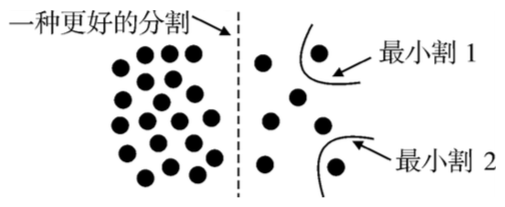
\includegraphics[width=0.5\textwidth]{minCuts.png}
\caption{最小割不一定是最优割的情况}
\label{fig: minCuts}
\end{figure} 

Ncut准则定义如下:
\begin{align}
\label{align: 类间的相关度}
Ncut(A, B) & = \frac{cut(A, B)}{assoc(A, V)} + \frac{cut(A, B)}{assoc(B, V)}\\
assoc(A, V) & = \sum_{u \in A, v \in V} w(u, v)
\end{align}

其中:$assoc(A, V)$是指子集$A$中所有节点到图中所有节点的边连接权重总和,$assoc(B, V)$也是类似的定义。这样定义两个区域之间的不相关性,使单个顶点分割的结果不再满足$Ncut$值最小,因此不会偏向分割单个孤立的顶点。

另外还定义了如下公式:
\begin{align}
\label{align: 类内的相关度}
Nassoc(A, B) = \frac{assoc(A, A)}{assoc(A, V)} + \frac{assoc(B, B)}{assoc(B, V)}
\end{align}

公式~(\ref{align: 类内的相关度})代表的是类内的相关度,它的值越大,分割效果越好。通过上面三个公式,可以将~(\ref{align: 类间的相关度})写成如下形式:
\begin{align}
\label{align: 类间类内}
Ncut(A, B) & = \frac{cut(A, B)}{assoc(A, V)} + \frac{cut(A, B)}{assoc(B, V)} \nonumber \\
          & = \frac{(assoc(A, V)-assoc(A, A)}{assoc(A, V)}+\frac{assoc(B, V)-assoc(B, B)}{assoc(B, V)} \nonumber \\
          & = 2 - (\frac{assoc(A, A)}{assoc(A, V)}+\frac{assoc(B, B)}{assoc(B,V)} \nonumber \\
          & = 2-Nassoc(A, B)
\end{align}

由式~(\ref{align: 类间类内})可知,$Ncut(A, B)$值越低表示相似度高的顶点分配到一个子图中,相似度低的顶点分配到不同子图中,是一种较理想的评价分割质量的标准。但由于$Ncut$被证明是$NP-hard$问题,且随着图中节点数目的增加,问题的求解变得异常复杂。在实际应用中,常把$Ncut$准则转换为矩阵计算的形式,并求解方程的特征值和特征向量。通常选择第二个最小特征值所对应的特征向量,它代表了图划分的最优解,并取一个合适的分裂点,将特征向量离散化为两个值,根据离散化后的值将图分割成两部分。如需要再细分,可以迭代地调用该算法进行二分。

\subsubsection{Ncut算法的求解}

假设一幅图$G = (V, E)$被分为$A$和$B$两部分,令$x$为一个$N = |V|$维指示向量,如果$x_i = 1$,则表明节点$i$在$A$中,如果$x_i= -1$,则表明节点$i$在$B$中。节点的度$d_i = \sum_j w(i, j)$是节点$i$与$V$中所有节点的关系之和。有了上面两个条件,可以将$Ncut(A, B)$写成如下式子:
\begin{align}
Ncut(A, B) & = \frac{cut(A, B)}{assoc(A, V)} + \frac{cut(A, B)}{assoc(B, V)} \nonumber \\
& = \frac{\sum_{(x_i>0, x_j<0)} -w_{ij}x_i x_j}{\sum_{x_i>0}d_i} + \frac{\sum_{(x_i<0, x_j>0)} -w_{ij}x_i x_j}{\sum_{x_i<0}d_i}
\end{align}

令$D$为$N \times N$对角矩阵,并且对角线上的元素为$d_i$,$w$为$N \times N$的对称矩阵,其元素值$W(i, j) = w(i, j)$,通过推到可将求解$Ncut(A, B)$最小值的问题转化为求解如下特征系统公式的第二小的特征向量:
\begin{align}
(\mathbf{D} - \mathbf{W})\mathbf{y} = \lambda \mathbf{Dy}
\end{align}

然后再将此特征向量离散化,就可以得到图像分割结果。

\subsubsection{Ncut算法的步骤}

1. 给定一幅图像,建立一个加权图,设定边的权值函数,用来度量两点间的相似程度。

2. 利用最小特征值求出对应的特征向量

3. 利用具有第二个最小特征值的特征向量$\mathbf{y}$来将图一分为二,在向量$\mathbf{y}$中选择一个分割数值(通常情况下选取0作为分割点),使$\mathbf{y}$中大于该数的部分所对应的节点在A中,其余的在$B$中。这样就可以将图像分割成两部分了。

4. 判断是否需要细分,如果有必要则可以采用递归方法将已分割的图再细分

存在的疑问:

1)如果图像是$300 \times 400$的,那么根据公式算出的特征向量就是$120000$维,对特征向量取阈值以对图像进行二分,会不会出现分成的连通区域不只两个的情况?


\subsection{Graph-based segmentation}

Felzenszwalb等人~\cite{felzenszwalb2004efficient}于2004年提出了一种基于图的超像素分割方法。主要是一种“小而合并”的思想。其代码见网站:\url{http://cs.brown.edu/~pff/segment/}

在图论中,树是任意两个顶点间有且只有一条路径的图。或者说,只要没有回路的连通图就是树。森林是指互相不交并树的集合。

算法输入:图像平滑参数$sigma$,阈值$k$,最小超像素大小$min$(由后处理阶段所限制),输入图像

算法输出:将图像分割成components $S = (C_1, \ldots, C_r)$

步骤:

1. 对输入彩色图像的每个颜色通道进行平滑,平滑的目的是compensate for digitization artifacts,可以使聚类中的像素点更紧密地连接在一起。

2. 将图像映射为图$G = (V, E)$:图像中每个像素点$p_i$看成是图上的一个节点$v_i$,相邻(8邻域)的两个节点之间的连线看成是图中的边,每条边都有对应的权重$w((v_i, v_j))$,这个权重值代表了相邻节点$v_i$和$v_j$之间的不相似度(例如在亮度、颜色、位置等属性上的不同),一般来说,每个节点有8条边,这篇论文中$w((v_i, v_j)) = |I(p_i)-I(p_j)|$,$I(p_i)$是像素点$p_i$上的亮度值。设图中一共有$n$个节点和$m$条边。

3. 分割:将图像分割成很多的components,要使同一component中的元素相似度较高,而使不同components中的元素的非相似度较高。也就是说,同一component中的节点之间的边应该有低的权值,而不同components中的节点之间的边应该有大的权值。

4. 对图中所有边按非递减的顺序进行排序,也就是将$E$中的边按非递减排成如下形式:$\pi = (o_1, \ldots, o_m)$。

5. 对排序后每条边,按非递减的顺序(从$q=1$到$q=m$),找到其连接的两个节点所属的component:最初的分割记为$S^0$,即每一个节点属于一个区域。由$S^{q-1}$构造$S^q$,记第$q$条边连接的两个节点为$v_i$和$v_j$,如果在$S(q-1)$中$v_i$和$v_j$是分别属于两个区域并且第$q$条边的权重小于两个区域的区域内间距,则合并两个区域。否则令$S^q = S^{q-1}$。

对彩色图像,要将这个算法运行三次,对r、g、b三通道分别运行一次,然后取这三组components的交集,也就是说,要判断两个相邻像素是否要归为同一component,需要其在三个色彩空间的分割效果都在同一component才行。当然,如果边的权重$w((v_i, v_j))$以及计算了两个节点在颜色空间的距离,那么算法就只需运行一次,但是实际实验效果显示将三个颜色空间的分割结果取交集效果会更好。


其中,定义区域内间距如下:
\begin{align}
Int(C) = \max_{c \in MST(C, E)}w(c)
\end{align}

\textbf{最小生成树}(minimum spanning tree, MST):在一个具有几个顶点的连通图$G$中,如果存在子图$G$'包含$G$中所有顶点和一部分边,且不形成回路,则称$G'$为图$G$的生成树,代价最小生成树则称为最小生成树。

定义区域间间距如下:
\begin{align}
Dif(C_1, C_2) = \min_{v_i \in C_1, v_j \in C_2, (v_i, v_j)\in E}w((v_i, v_j))
\end{align}

定义$D(C_1, C_2)$来评价在一次分割中的两个components之间是否有存在边界的迹象。
\begin{equation}
 D(C_1, C_2)= \left\{
    \begin{array}{rl}
      true & \text{如果} Dif(C_1, D_2) > MInt(C_1, C_2)\\
      false & \text{其它情况}
    \end{array} \right.
\end{equation}

其中,
\begin{align}
MInt(C_1, C_2) = min(Int(C_1)+\tau(C_1), Int(C_2)+\tau(C_2))
\end{align}

此处的$\tau$是一个阈值函数,用来控制两个区域的区域间间距要在多大程度上大于他们的区域内间距才能被认定为两个区域间有明显的分割界限。举个例子来说,当其中一个区域很小时,$Int(C)$并不能很好的反应其区域内间距(极端的情况是当$C$只含一个节点时,$Int(C)=0$)。这篇论文中在此处对$\tau$的定义为$|C|$的负相关函数:
\begin{align}
\tau(C) = k/|C|
\end{align}

其中$|C|$表示$C$的大小,也就是$C$中元素的个数。$k$是一个常数,$k$要根据实验的具体情况来确定其值,一开始,每个区域中只有一个节点,区域尺寸较小,因而判断两个区域间有无边界需要一个较强的约束,不然的话大多数区域都会不合并。$k$越大,我们界定的可以区分两个区域的界限就越明显,这样最终分割出的超像素区域会相对较大。所以$k$应该取决于图像的分辨率大小以及场景中对于细节的要求程度。这里$k$并不是分割出的component的最小尺寸,尺寸比$k$值小的components是允许的,只要此区域与相邻区域相比区域间间距较大,就不会被合并。

6. 后续对小的components进一步处理

7. 对每个component挑选一种随机颜色用来表示以区分于其他components

Graph-based方法通过将图上的节点进行聚类来实现,且生成的超像素就是像素集合的最小生成树。整个分割结果就是由一些不相交的最小生成树组成的森林。


\section{基于梯度上升的超像素分割方法}

梯度上升方法是从一个粗糙的像素的初始聚类开始,通过不断的迭代来优化聚类簇,直至满足收敛准则以形成超像素。以下几种方法都采用了聚类的基本思想,但各自具体方法不同,也有不同的优缺点。

\subsection{Mean shift算法}

\subsubsection{概念}

代码见网站:\url{http://www.vlfeat.org/download/}。

1. 看了百度文库上的这篇文章~\cite{MeanShiftIntroduction}后的几点收获:

1)Mean shift有两种含义,早期刚提出时Mean shift是一个名词,指代的是偏移的均值向量。而我们现在所说的Mean shift通常是一个动词,指的是一个迭代的步骤,即先算出当前点的偏移均值,移动该点到其偏移均值,然后以此为新的起始点,继续移动,直到满足一定的条件结束。

2)几个难懂而又关键的词语:Mean shift向量、核函数、核密度估计、带宽矩阵

\subsubsection{原理}

1975年Fukunage在论文\cite{fukunaga1975estimation}中首先提出Mean shift的概念,这篇论文主要是估计样本数据的多元概率密度梯度,基本思想是:某点的概率密度梯度可以用其周围一个很小的区域内的样本观测值来估计。对样本中的每一点,需要估计出其周围$k$个点的梯度向量,$k$是固定的,这些梯度向量就叫做“k最近邻Mean shift簇",对这些Mean shift向量求加权平均则得到该点的密度梯度。

1995年由Cheng发表的文献中定义了核函数和权值函数,使Mean shift算法得到了广泛应用。

设$X_1, X_2, \cdots, X_N$是一组由$N$个独立同分布的$n$维随机向量组成的集合。在$X$点处密度梯度表示如下:
\begin{align}
\label{align: DensityGradient}
\hat{\bigtriangledown}_x p_N(X) = (Nh^{n+2})^{-1}2c \sum_{X_i \in S_h(X)} (X_i - X) = \left(\frac{k}{Nv_h(X)}\right) \frac{n+2}{h^2} \left(\frac{1}{k} \sum_{X_i \in S_h(X)} (X_i - X)\right)
\end{align}

其中,
\begin{align}
v_h(X) \equiv \int_{S_h(X)}dY = \frac{h^n\pi^{n/2}}{\Gamma(n+2/2)}\\
S_h(X) \equiv \{Y:(Y-X)^T(Y-X) \le h^2\}
\end{align}

Mean shift向量就是从密度函数梯度的非参数估计中推导获得的,取~(\ref{align: DensityGradient})式的最后一项就是就是Mean shift向量
\begin{align}
M_h(X) \equiv \frac{1}{k} \sum_{X_i \in S_h(X)} (X_i-X)
\end{align}

显然,如果梯度为零,对应$S_h(X)$区域内密度较均匀,$X$处的偏移的均值向量也将为零;如果$X$处的密度梯度是一个指向概率密度函数增长最快的方向的非零梯度,那么从平均意义上说,$X$周围更多的观测点都将沿其方向存在,相应地,偏移的均值向量Mean shift也应该指向该方向,并且其长度与梯度大小成比例。

举个例子,见\cite{MeanShiftExample}

在$d$维空间中,任选一个点,然后以这个点为圆心,$h$为半径作一个高维球。落在这个球内的所有点和圆心都会产生一个向量,向量是以圆心为起点落在球内的点位终点,然后把这些向量都相加,相加的结果就是Mean shift向量。如图~\ref{fig: meanshift1}所示,其中黄色箭头就是Mean shift向量。

\begin{figure}[!ht]
\centering
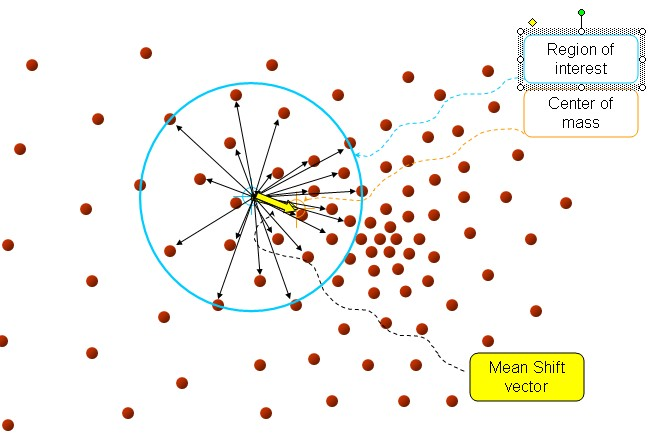
\includegraphics[width=0.5\textwidth]{meanshift1.jpg}
\caption{初始状态}
\label{fig: meanshift1}
\end{figure} 


再以Mean shift向量的终点为圆心,再做一个高维的球。如图~\ref{fig: meanshift2}所示,重复以上步骤,就可得到一个Mean shift向量,如此重复下去,可以收敛到概率密度最大的地方,也就是最稠密的地方。

\begin{figure}[!ht]
\centering
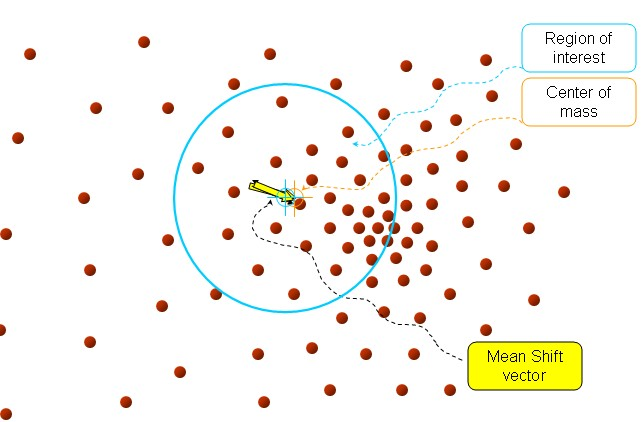
\includegraphics[width=0.5\textwidth]{meanshift2.jpg}
\caption{迭代过程}
\label{fig: meanshift2}
\end{figure} 

最终结果如图~\ref{fig: meanshift3}。

\begin{figure}[!ht]
\centering
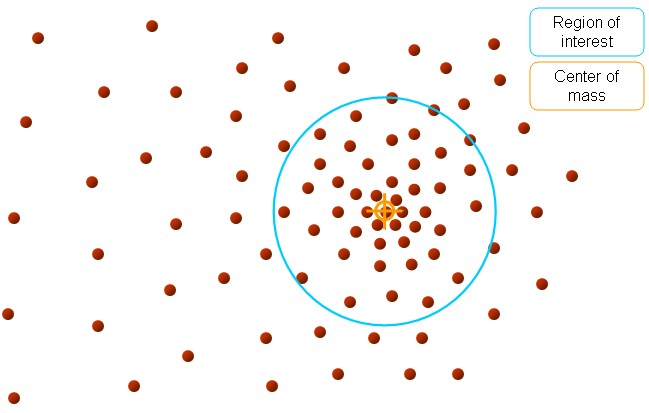
\includegraphics[width=0.5\textwidth]{meanshift3.jpg}
\caption{最终状态}
\label{fig: meanshift3}
\end{figure} 

应用到图像分割中:需要将图像映射到特征空间中,例如映射到颜色特征空间,图像分割就是求每一个像素点的类标号。类标号取决于它在特征空间所属的cluster。对于每一个cluster,首先得有个类中心,它深深地吸引着一些点,就形成了一个类。

需要解决的问题有两个,what:中心是什么?how:怎么找?Mean shift认为中心是概率密度的极大值点。对于每个点,怎么找到它的类中心呢?只要沿着梯度方向一步一步慢慢爬,就总能爬到极值点。不过一般的梯度上升方法并不能保证收敛到局部极大值,但Mean shift可以做到,因为它的步长是自适应调整的,越靠近极值点步长就越小。

2. 经学习后对上述词语的理解: 

\textbf{核密度估计}:由给定样本点集合求解随机变量的分布密度函数问题是概率统计学的基本问题之一。解决这一问题的方法包括参数估计和非参数估计。其中非参数估计又有直方图估计、核密度估计等。

核密度估计方法是由Rosenblatt~\cite{rosenblatt1956remarks}和Parzen~\cite{parzen1962estimation}提出的,该方法不利用有关数据分布的先验知识,对数据分布不附加任何假定,是一种从数据样本本身出发研究数据分布特征的方法。

核密度估计的目的:设$x_1, x_2, \ldots, x_n$是从具有未知密度函数$f(x)$的总体中抽出的独立同分布样本,要依据这些样本对每一$x$去估计$f(x)$的值。

核密度估计的公式为:

\begin{align}
\hat{f}(x) = \frac{1}{nh}\sum_{i=1}{n}K(\frac{x-x_i}{h})
\end{align}

其中K(.)称为\textbf{核函数},满足对称性及$\int K(x)dx=1$。

$h$称为带宽,一般$h$越大,估计的密度函数就越光滑,但偏差可能较大,选择的原则是使得均方误差最小。在实际中,带宽的选择很大程度上取决于主观判断:如果认为真实的概率密度分布曲线是比较平坦的,那么就选择较大的带宽;相反,如果认为真实的概率分布曲线是比较陡峭的,那么就选择较小的带宽。

核密度估计原理:利用数据点$x_i$到$x$的距离来决定$x_i$在估计点$x$的密度时所起的作用,若某个数在观察值中出现了,我们可以认为这个数的概率密度比较大,和这个数比较近的数的概率密度也会比较大,而那些离这个数远的数的概率密度会比较小。基于这种想法,对点$x$来说,若$x-x_i$较小,说明$x$与观测值$x_i$相距较近,因而$x$处的概率密度也会比较大,若$x-x_i$较大,则对应$x$处的概率密度也会比较小,可以用$\cfrac{1}{h}K\left(\cfrac{x-x_i}{h}\right)$来拟合我们想象中的那个远小近大的概率密度,其中K函数内部的h分母用于调整KDE曲线的宽幅,而K函数外部的h分母则用于保证曲线下方的面积符合KDE的规则(KDE曲线下方面积和为1)。针对每一个观察中出现的数拟合出多个概率密度分布函数之后,取平均。



\subsubsection{应用}

1. 聚类

Mean shift算法是基于概率密度的方法,不需要任何先验条件,数据集中的每一点都可以作为初始点,分别执行Mean shift算法,收敛到同一个点算作一类,它能对任何维度、任何分布的采样点进行聚类。

2. 图像分割

Mean shift算法是一种统计聚类方法,在图像分割时,首先将图像像素转换成特征空间的采样点,例如対一幅彩色图像,考虑到图像的空间信息和色彩信息,特征空间可由2维的位置空间和3维的色度空间组成,图像像素转换成特征空间中的一个5维采样点,然后对采样点进行Mean shift聚类,特征空间中的聚类对应于图像空间的分割。

3. 目标跟踪

利用Mean shift算法进行物体跟踪的实质是求解最优化的Bhattacharrya系数函数\cite{fashing2005mean}。该函数表示的是目标对象和候选对象的相似度,通过泰勒展开后可转化为隐含估计的概率密度函数,因此用Mean shift算法求解。

\subsection{TurboPixels}

2009年Levinshtein等人~\cite{levinshtein2009turbopixels}采用了一种基于几何流的水平集方法,能快速地产生超像素。该方法来源于早期计算机视觉领域中的曲线演化技术。通过膨胀初始化种子点,并结合曲率演化模型和背景区域的骨架化过程,将图像分割为网格状的超像素。代码见网站:\url{http://www.cs.toronto.edu/~babalex/turbopixels_supplementary.tar.gz.}。

\textbf{几何流}:几何流的概念来自微分几何。与某种几何特性有关的一类偏微分方程称为几何偏微分方程。几何曲线(曲面)在几何偏微分方程的驱动下发生变形的过程,类似于热传导,通常称为几何热流,简称几何流(Geometric Flows)~\cite{sapiro2006geometric, bakas2005algebraic}。通常直接将这种几何偏微分方程称为几何流。

\textbf{曲线演化理论}:人们对曲线演化的研究起源于对晶体生长、火焰燃烧等物理现象的边界跟踪~\cite{sethian1985curvature}。

\textbf{Level Set方法}:Level Set方法是加州大学数学家Osher(洛杉矶分校)和Sethian(伯克利分校)合作提出的~\cite{osher1988fronts}。其基本思想是:将运动的轮廓曲线(曲面)隐含地表达为高一维的曲面(水平集函数)的零水平集,并通过曲面的运动来隐含地求解轮廓曲线(曲面)的演化。

TurboPixels生成的超像素遵循五个基本原则:

1)均匀尺寸:算法应把图像分为尺寸和形状大致相同的超像素,可以通过设计几何流来膨胀初始均匀分布的种子达到此目的

2)连通性:每个超像素应该表示一个简单连通的像素集合,采用结合水平集的几何流扩张方法能确保此约束总是满足

3)紧凑性:为了使超像素最大限度地紧凑,需要使强度均匀的区域在法线向外方向产生恒定的运动

4)平滑和边缘保持:当种子增长停止时,超像素边界应该和图像边界相吻合,这需要几何流公式在边界强度弱或者没有边界的地方,曲线运动速度大,而边界强度较强的地方,曲线速度慢甚至停止,从而实现图像的分割

5)超像素不重叠:算法应该把每个像素分配到单一超像素中。因此,当两个不同的种子膨胀到即将碰撞时,应该停止边界增长

基本步骤:

1)指定要分割的超像素个数$K$,将图像均分为$K$个网格,每个网格中放置一个初始种子点。

2)由于图像并不是均匀分布的,所以初始种子点可能会落在图像上的边界处,为了解决这个问题,可将种子点的位置打乱,使其远离梯度值较高的区域。

3)迭代以下步骤,直至不再有进一步的演化
 
a)第$T$次演化边界

b)估计未分配区域的骨架

c)更新边界上像素点的速度和在边界附近未分配像素点的速度

\subsection{SLIC算法}

SLIC是Simple Linear Iterative Clustering的缩写,最早由Achanta~\cite{achanta2010slic}于2010年6月在洛桑联邦理工学院的一次技术报告中提出。2012年经整理、完善后发表在TPAMI上~\cite{achanta2012slic}。其中“Linear”体现在算法复杂度$O(N)$与图像中像素个数$N$是线性关系,“Clustering"是采用k-均值聚类。代码见网站:\url{http://www.vlfeat.org/download/}。

k均值聚类:“k”表示将给定的数据划分为k个聚类,“均值”体现在更新聚类中心时,要分别计算k个聚类中的样本均值向量。主要思想:

(1)首先由用户随机(任意)指定需要划分的聚类数目k,然后选取k个初始聚类中心(初始聚类中心可以任意选取,也可以通过一定的方法进行选取,例如通过观察数据集中前几个值进行选取)

(2)对给定数据中的每一个点,计算到这k个聚类中心的距离,到哪个聚类中心的距离最小,这个点就属于哪一类。

由此就得到了一个初始的划分,之后

(3)更新聚类中心为该类中所有样本的均值向量

(4)重复步骤(2)和(3),直至聚类中心不再发生变化,迭代结束。

SLIC是一种使用简单和易于理解的方法,是对传统的k-均值超像素分割方法的改进,类似于quick shift与mean shift之间的关系。两者之间主要有以下两点区别:

1. SLIC优化了距离计算的数目,传统的k-均值方法中每个聚类中心的搜索范围是整幅图像,要计算该聚类中心与图像中所有像素点之间的距离,而SLIC算法只在与预设的超像素尺寸成比例的一个区域内搜索,见图~\ref{fig: searchregion}。

\begin{figure}[!ht]
\centering
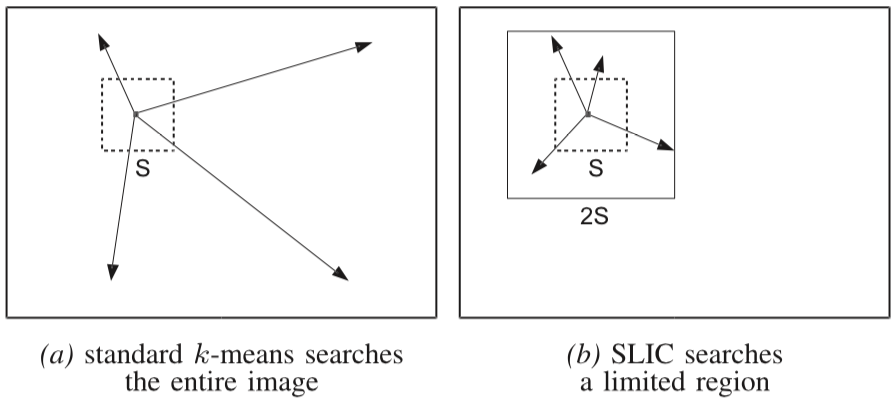
\includegraphics[width=0.7\textwidth]{searchregion.png}
\caption{传统的k-均值方法与SLIC算法搜索区域的区别}
\label{fig: searchregion}
\end{figure} 

2. SLIC算法在计算聚类中心与像素点之间的距离时同时结合了颜色和空间位置两方面的信息来表征其相似度,这样可以起到控制超像素尺寸和紧密度的作用。

默认情况下,该算法只有一个参数$k$,即所需生成的近似同样大小的超像素的个数。具体步骤为:

a)初始化聚类中心。假设一幅彩色图像有$N$个像素点,预分割为$k$个相同尺寸的超像素,那么首先要将该彩色图像转换为CIELAB颜色空间和XY坐标下的5维特征向量,然后将图像均分为$k$个网格,网格边长为$S=\sqrt{N/k}$,k个初始聚类中心$C_i=[l_i, a_i, b_i, x_i, y_i]^T$为每个网格内色阶值最低的像素。对图像中的每一个像素点,令其与最近的聚类中心的距离$d(i)$的初始值为$\infty$。

b)相似度衡量。对于每个聚类中心,逐一计算其$2S \times 2S$邻域内(如图~\ref{fig: searchregion})各像素$i$与该类中心点的距离$D$,若$D<d(i)$,则$i$暂时归为该类,并且将$d(i)$赋值为$D$,其中
\begin{align}
d_c & =  \sqrt{(l_j-l_i)^2+(a_j-a_i)^2+(b_j-b_i)^2}\\
d_s & =  \sqrt{(x_j-x_i)^2+(y_j-y_i)^2}\\
D & =  \sqrt{d_c^2+\left(\frac{d_s}{S}\right)^2m^2}
\end{align}

c)确定新的聚类中心。当每个像素都被归类到其最近的聚类中心后,新的聚类中心为该类中所有像素的$[l, a, b, x, y]^T$向量的平均值。为了避免聚类中心落在边界上,以及对后续的聚类过程造成干扰,需要将聚类中心在以$3\times3$的邻域内打乱,将聚类中心移到邻域内梯度最小的地方(图像灰度值变化最缓慢的地方)。计算残差$E$(新的聚类中心与之前聚类中心的$L1$范数)。

d)重复b)和c)直至最后收敛($E\le threshold$)。

\section{实验效果分析}

Graph-based segmentation、Ncut、QuickShift、TurboPixels、SLIC方法的效果分别如图~\ref{fig: GB}、~\ref{fig: Ncut}、~\ref{fig: QuickShift}、~\ref{fig: TurboPixels}、~\ref{fig: SLIC}。

\begin{figure}
  \centering 
  \subfigure[]{ 
    \label{fig: GB: a} %% label for first subfigure 
    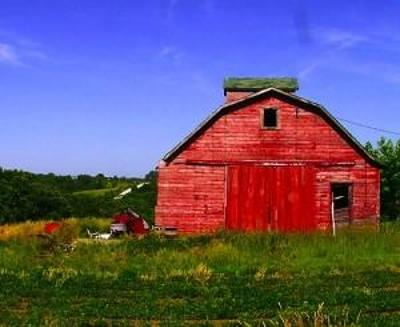
\includegraphics[width=0.4\textwidth]{example1.jpg}} 
  \subfigure[]{ 
    \label{fig: GB: b} %% label for second subfigure 
    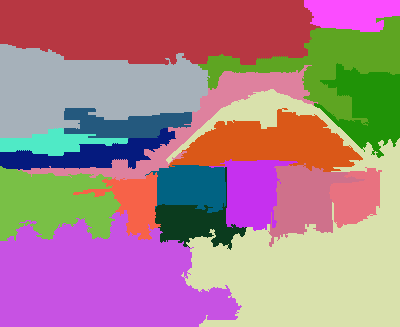
\includegraphics[width=0.4\textwidth]{GB1.png}} 
  \caption{Graph-based segmentation: sigma = 0.3, k = 350, min = 1200}
  \label{fig: GB} %% label for entire figure 
\end{figure}

\begin{figure}
  \centering 
  \subfigure[]{ 
    \label{fig: Ncut: a} %% label for first subfigure 
    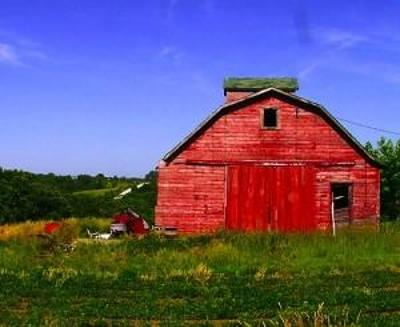
\includegraphics[width=0.4\textwidth]{example1.jpg}} 
  \subfigure[]{ 
    \label{fig: Ncut: b} %% label for second subfigure 
    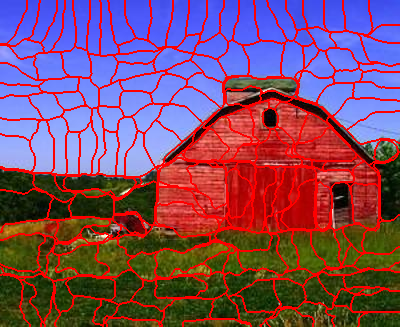
\includegraphics[width=0.4\textwidth]{Ncut1.png}} 
  \caption{Ncut: $N_{sp}$ = 200}
    \label{fig: Ncut} %% label for entire figure 
\end{figure}

\begin{figure}
  \centering 
  \subfigure[]{ 
    \label{fig: QuickShift: a} %% label for first subfigure 
    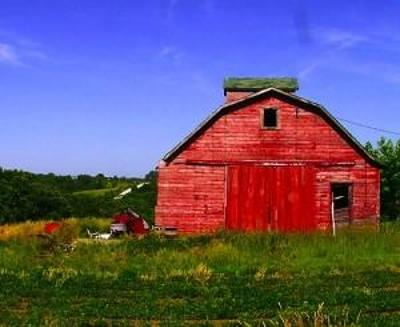
\includegraphics[width=0.4\textwidth]{example1.jpg}} 
  \subfigure[]{ 
    \label{fig: QuickShift: b} %% label for second subfigure 
    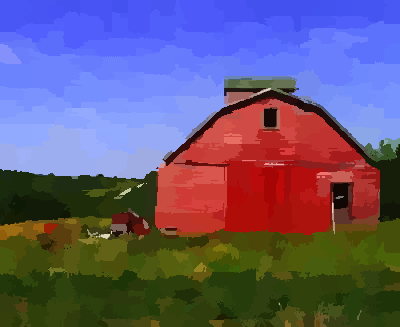
\includegraphics[width=0.4\textwidth]{QuickShift1.png}} 
  \caption{QuickShift: ratio = 0.5, kernelsize = 2, maxdist = 10}
  \label{fig: QuickShift} %% label for entire figure 
\end{figure}

\begin{figure}
  \centering 
  \subfigure[]{ 
    \label{fig: TurboPixels: a} %% label for first subfigure 
    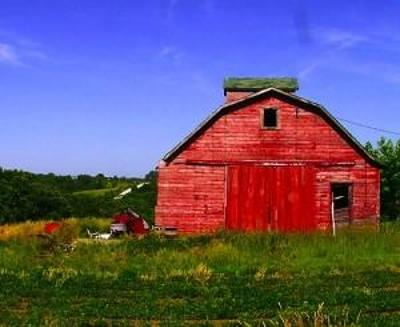
\includegraphics[width=0.4\textwidth]{example1.jpg}} 
  \subfigure[]{ 
    \label{fig: TurboPixels: b} %% label for second subfigure 
    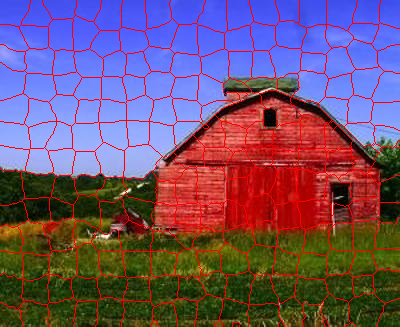
\includegraphics[width=0.4\textwidth]{TurboPixels1.png}}  
  \caption{TurboPixels: $N_{sp}$ = 200}
  \label{fig: TurboPixels} %% label for entire figure
\end{figure}

\begin{figure}
  \centering 
  \subfigure[]{ 
    \label{fig: SLIC: a} %% label for first subfigure 
    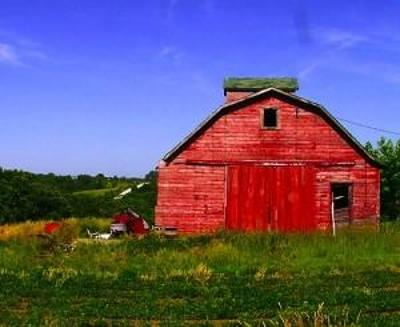
\includegraphics[width=0.4\textwidth]{example1.jpg}} 
  \subfigure[]{ 
    \label{fig: SLIC: b} %% label for second subfigure 
    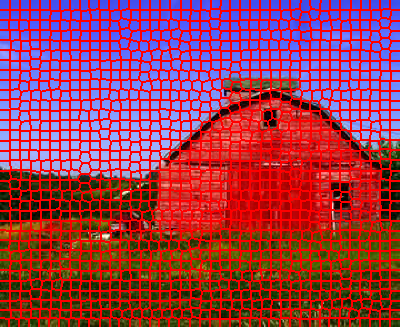
\includegraphics[width=0.4\textwidth]{SLIC1.png}} 
  \caption{SLIC: regionSize = 10, regularizer = 10}
  \label{fig: SLIC} %% label for entire figure 
\end{figure}

\begin{table}[!h] %插表
\label{tab: 1}
\centering
\begin{tabular}{|c|c|c|c|c|c|}
\hline
$\quad$ & Graph-based & Ncut & Mean shift & TurboPixels & SLIC \\
\hline
是否可控制超像素的数目 & 否 & 是 & 否 & 是 & 是\\
\hline
运行时间($327 \times 400$图像)& 1.470s & 78.188s & 1.377s & 9.493s & 0.314s\\
\hline
\end{tabular}  
\caption{对比}
\end{table}
%
% references
\bibliographystyle{plain}

\bibliography{superpixel} %参考文献


%%---------------------------------------------------------------------
\end{document}
